\documentclass{beamer}
\usepackage{graphicx} % Required for inserting images
\usepackage[utf8]{inputenc}
\usepackage{enumitem}
\usepackage{amsmath}
\usepackage{listings}
\usepackage{xcolor}

\definecolor{codegreen}{rgb}{0,0.6,0}
\definecolor{codegray}{rgb}{0.5,0.5,0.5}
\definecolor{codepurple}{rgb}{0.58,0,0.82}
\definecolor{backcolour}{rgb}{0.95,0.95,0.92}

\lstdefinestyle{mystyle}{
    backgroundcolor=\color{backcolour},   
    commentstyle=\color{codegreen},
    keywordstyle=\color{magenta},
    numberstyle=\tiny\color{codegray},
    stringstyle=\color{codepurple},
    basicstyle=\tiny\ttfamily,
    breakatwhitespace=false,         
    breaklines=true,                 
    captionpos=b,                    
    keepspaces=true,                 
    numbers=left,                    
    numbersep=5pt,                  
    showspaces=false,                
    showstringspaces=false,
    showtabs=false,                  
    tabsize=2
}

\lstset{style=mystyle}

\usetheme{Madrid}
\usecolortheme{default}

\title{Modélisation de l'évolution de la température}
\subtitle{Approche par un automate cellulaire.}
\author{Huet Natanéo \and Hurot Eliott} 
\date{2024}
\logo{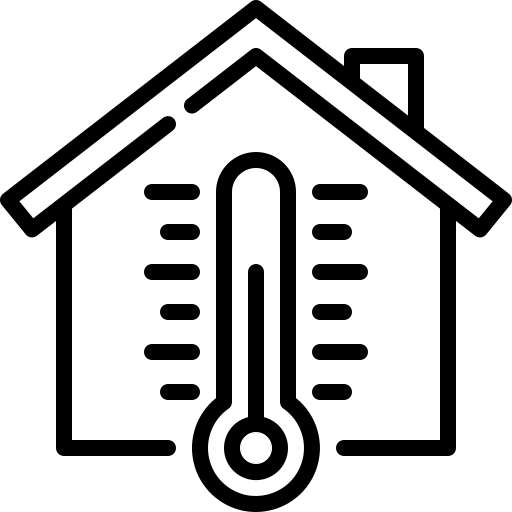
\includegraphics[height=1cm]{room-temperature.png}}

\begin{document}

\frame{\titlepage}

\begin{frame}{Problématique}
    \begin{center}
        \huge{Comment modéliser l'évolution de la \\ température d'une maison via un \\ automate cellulaire ?}
    \end{center}
\end{frame}

\begin{frame}
    \frametitle{Sommaire}
    \tableofcontents
\end{frame}

\section{Définition d'automate cellulaire}
\begin{frame}
    \frametitle{Définition d'automate cellulaire}

    4-uplet $ ( d, Q, V, \delta ) $ 
    \begin{itemize}
        \item $d$ est la dimension
        \item $Q$ est l'alphabet
        \item $V$ est le voisinage
        \item ${ \delta : Q^{\alpha} \longrightarrow Q }$ est la règle de transistion
    \end{itemize}
\end{frame}

\section{Premier modèle}
\begin{frame}
    \frametitle{Premier modèle}
    \begin{align*}
    & \Delta U = W + Q \\
    & C_v \Delta T_{cellule} = W + Q \\
    & \delta Q = \phi \Delta t \\
    & \Delta T_{difference} = \phi R_{th} \\
    & \Delta T_{cellule} = \frac{\Delta T_{difference} \times \Delta t} {R_{th} \times C_v} 
    \end{align*}
    
\end{frame}

\begin{frame}[fragile]
    \frametitle{Définition des structures}

    \begin{lstlisting}[
        language=C
    ]
struct cell
{
    float T; // --------------- en degre Celsius
    char* type; // ------------ type de la cellule (airExt, airInt, wall, window, door)
    coord co; // -------------- coordonnees de la cellule
    float CTherVol; // -------- Capacite thermique volumique en J.K-1.m-3
    float lambda; // ---------- Conductivite thermique en W.K-1.m-1
    float surface; // --------- Surface en m2
    float epaisseur; // ------- Epaisseur en m
    float lambda_iso_ext; // -- Conductivite thermique de l'isolant exterieur en W.K-1.m-1
    float lambda_iso_int; // -- Conductivite thermique de l'isolant interieur en W.K-1.m-1
    float epaisseur_iso_ext; // Epaisseur de l'isolant exterieur en m
    float epaisseur_iso_int; // Epaisseur de l'isolant interieur en m
};
    \end{lstlisting}

\end{frame}

\begin{frame}[fragile]
    \frametitle{Définition des structures}
    
    \begin{lstlisting}[
        language=C
    ]
struct cell
{
    float T; // --------------- en degre Celsius
    char* type; // ------------ type de la cellule (airExt, airInt, wall, window, door)
    coord co; // -------------- coordonnees de la cellule
    float CTherVol; // -------- Capacite thermique volumique en J.K-1.m-3
    float lambda; // ---------- Conductivite thermique en W.K-1.m-1
    float surface; // --------- Surface en m2
    float epaisseur; // ------- Epaisseur en m
    float lambda_iso_ext; // -- Conductivite thermique de l'isolant exterieur en W.K-1.m-1
    float lambda_iso_int; // -- Conductivite thermique de l'isolant interieur en W.K-1.m-1
    float epaisseur_iso_ext; // Epaisseur de l'isolant exterieur en m
    float epaisseur_iso_int; // Epaisseur de l'isolant interieur en m
};
    \end{lstlisting}
    
\end{frame}

\begin{frame}[fragile]
    \frametitle{Exemple de structure}
    
    \begin{lstlisting}[
        language=C
    ]
 structure window1 = {
    .T = 10.0,
    .type = "window",
    .begining = {.i = 2, .j = 8},
    .ending = {.i = 2, .j = 10},
    .CTherVol = 17000,
    .lambda = 1.0,
    .surface = 2.0,
    .epaisseur = 0.1,
};
    \end{lstlisting}
\end{frame}

\begin{frame}
    \frametitle{Règles de l'automate cellulaire}

    L'air ext est constant. \\[0.5cm]
    Pour tout le reste des cellules du modèle on calcule $Q$ en fonction des 4 cellules adjacentes à celle que l'on regarde.\\[0.5cm]
    Pour l'air int on calcule $Q$ avec les résistances termiques des cellules d'air adjacentes.

\end{frame}

\begin{frame}
    \frametitle{Fonction de Transfert}
    \begin{figure}
        \centering
        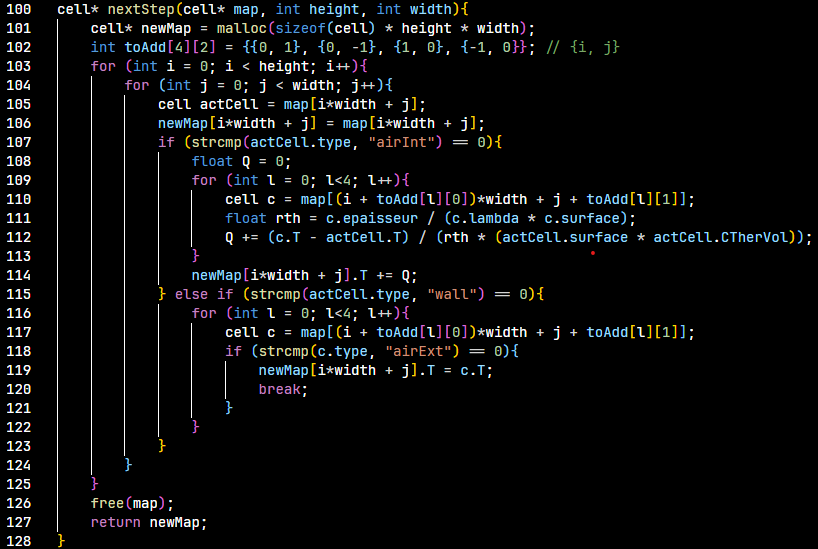
\includegraphics[width=12cm, height=8cm]{nextStep.png}
        \label{fig:nextStep}
    \end{figure}
\end{frame}

\section{Premier résultat}
\begin{frame}{Validation du premier modèle}
    \begin{figure}
        \centering
        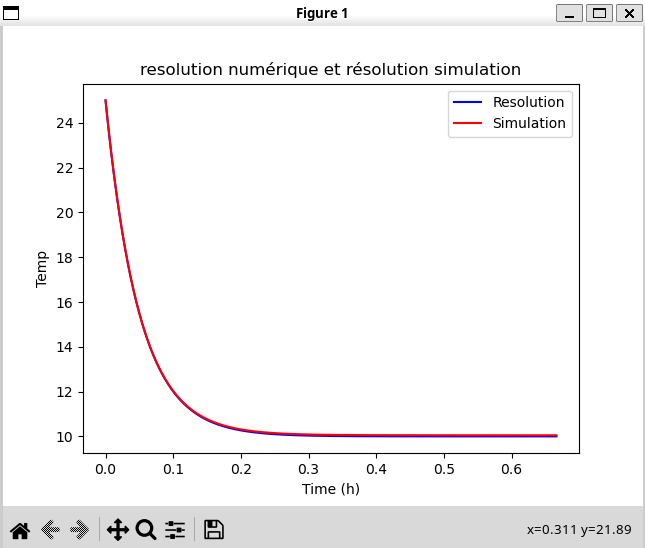
\includegraphics[width=10cm, height=7cm]{courbe.png}
        \label{fig:courbe}
    \end{figure}
\end{frame}

\section{Ajout de la convection}
\begin{frame}{Problème soulevé}
    \begin{figure}
        \centering
        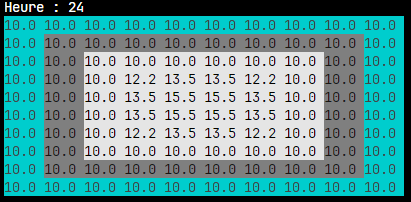
\includegraphics[width=12cm]{compilation.png}
        \label{fig:compilation}
    \end{figure}
\end{frame}

\begin{frame}{Solution}
    Présence d'un ventilateur homogénisant la pièce : \ref{fig:convection}
    \begin{figure}
        \centering
        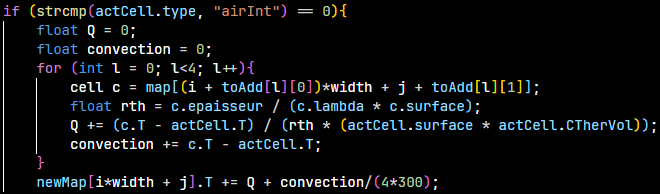
\includegraphics[width=10cm]{convection.png}
        \caption{Fonction nextStep mise à jour}
        \label{fig:convection}
    \end{figure}    
\end{frame}

\begin{frame}{Résultats}
    \begin{figure}
        \centering
        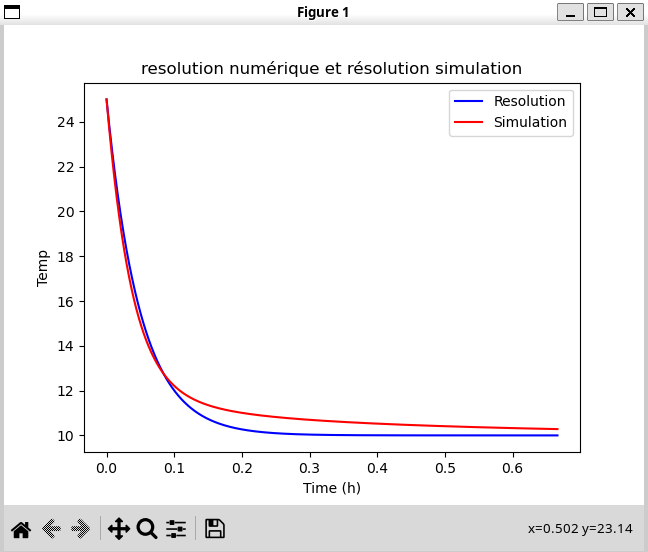
\includegraphics[width=10cm, height=7cm]{courbe2.png}
        \label{fig:courbe2}
    \end{figure}
\end{frame}

\begin{frame}
    \begin{figure}
        \centering
        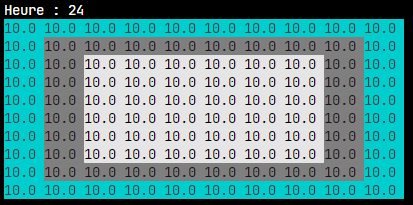
\includegraphics[width=12cm]{compilation2.png}
        \label{fig:compilation2}
    \end{figure}
\end{frame}

\section{Modèle final}
\begin{frame}
    \frametitle{Modèle final}

    \[ 
    \Delta T_{cellule} = \frac{\Delta T_{difference} \times \Delta t} {R_{th} \times C_v} 
    \]
    \\[1cm]
    Ici, on différencie l'isolation intérieur de l'extérieur.\\
    Cela permet aussi de donner aux murs leurs propre température. 
    \\[1cm]
    On note aussi l'ajout d'autres structures telles que les portes ou les fenêtres, ayant leurs propres $C_v$, $\lambda$, etc.
    
\end{frame}

\begin{frame}
    \begin{figure}
        \centering
        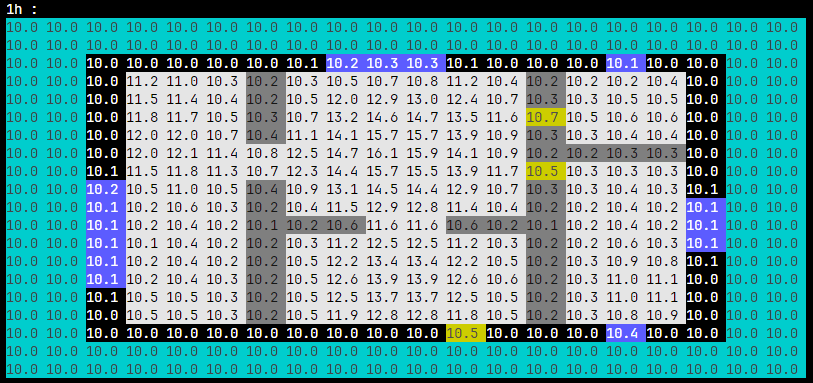
\includegraphics[width=12cm]{compilation3.png}
        \label{fig:compilation3}
    \end{figure}
\end{frame}

\begin{frame}[fragile]
\frametitle{Programmation}
    \begin{lstlisting}[
        langage=C
    ]
else if (strcmp(actCell.type, "isolated wall") == 0)
    {
        float Q = 0;
        for (int l = 0; l < 4; l++){

            if (i+toAdd[l][0] >= 0 && i+toAdd[l][0] < height && j+toAdd[l][1] >= 0 && j+toAdd[l][1] < width){
                cell c = map[(i+toAdd[l][0])*width + j+toAdd[l][1]];
                
                if (strcmp(c.type, "airInt") == 0)
                {
                    Q += (c.T - actCell.T) * 1 / ((actCell.epaisseur_iso_int / (actCell.lambda_iso_int * actCell.surface)) * actCell.CTherVol * actCell.surface * actCell.epaisseur);
                }
                else if (strcmp(c.type, "airExt") == 0)
                {
                    Q += (c.T - actCell.T) * 1 / ((actCell.epaisseur_iso_ext / (actCell.lambda_iso_ext * actCell.surface)) * actCell.CTherVol * actCell.surface * actCell.epaisseur);
                }
                else
                {
                    Q += (c.T - actCell.T) * 1 / ((c.epaisseur / (c.lambda * c.surface)) * actCell.CTherVol * actCell.surface * actCell.epaisseur);
                }
            }

        }
    \end{lstlisting}
\end{frame}



\begin{frame}{Observation}
    \begin{figure}
        \centering
        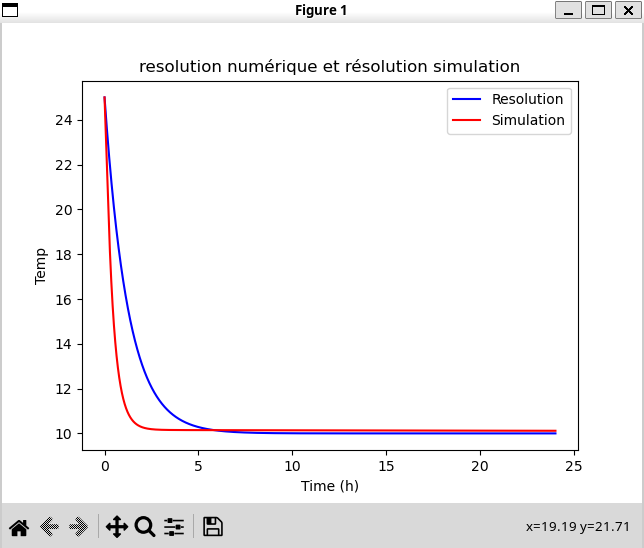
\includegraphics[width=10cm, height=7cm]{courbe3.png}
        \caption{Température initial des murs à 10°C}
        \label{fig:courbe3}
    \end{figure}
\end{frame}

\begin{frame}
    \begin{figure}
        \centering
        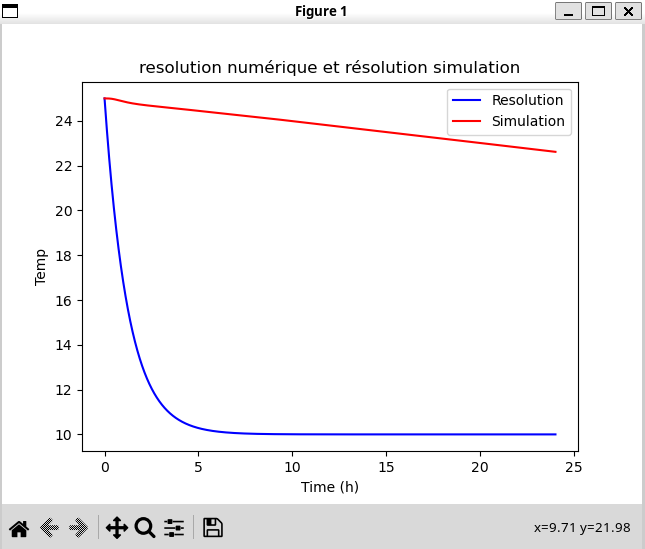
\includegraphics[width=10cm, height=7cm]{courbe4.png}
        \caption{Température initial des murs à 25°C}
        \label{fig:courbe4}
    \end{figure}
\end{frame}

\begin{frame}
    \frametitle{Ajout du chauffage et autres structures}

    \begin{cases}
        \Delta T_{cellule} = \frac{P \times \Delta t}{C_{v}} \text{ si } T_{cellule} < \text{18C} \\
        \text{Aucun chauffage sinon}
    \end{cases}
    
\end{frame}

\begin{frame}
    \begin{figure}
        \centering
        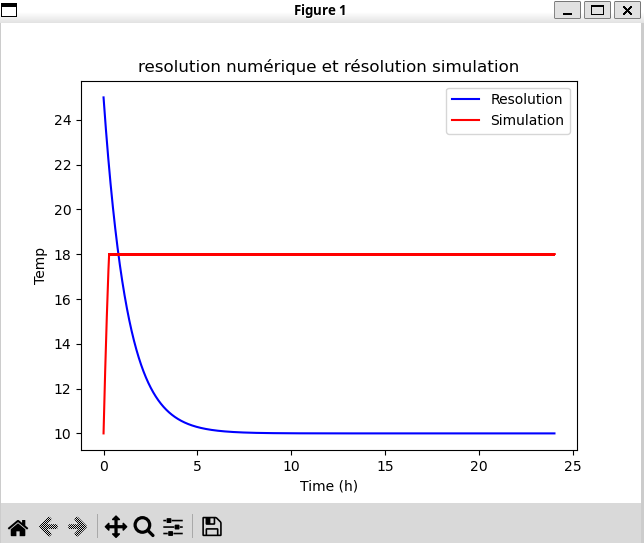
\includegraphics[width=10cm]{courbe5.png}
        \label{fig:courbe5}
    \end{figure}
\end{frame}

\section{Objectifs}
\begin{frame}{Objectifs}
    \begin{itemize}
        \item Réduire les suppositions (loi de newton, pont thermique...)
        \item Ajout des plages de chauffage
        \item Ajout d'une troisième dimension
        \item Précision de la problématique
    \end{itemize}
\end{frame}

\end{document}